% TODO: ПОМЕНЯЙТЕ НА СВОЙ ПУТЬ ПРИ СБОРКЕ
\renewcommand{\mainFolder}{/home/aleksei/github_projects/latex_works/informatics}
\renewcommand{\myFolder}{\mainFolder/lecture_\arabic{lectureNo}/}

%	LECTURE INFO
%----------------------------------------------------------------------------------------
\renewcommand{\lectureSubject}{Типы в C++}
%----------------------------------------------------------------------------------------
%
% Главное - указывать в путях для добавляемых файлов переменную \myFolder.
% Так, новый cpp файл должен иметь путь \cppfile{\myFolder/main}{....} (указывается без расширения)
% Нельзя писать \cppfile{main}{...} !!!
% Если не выполнить это требование, большой проект не будет собираться


\begin{lecture}[\lectureSubject]
	\begin{lecSection}[Строгая статическая типизация в C++]
		Проверка типов происходит в \underline{момент компиляции}.
		\cppfile{\myFolder/1}{Неправильное присваивание}{1}
		Помимо этого, присваивание является арифметической операцией (делает дело и возвращает число).
	\end{lecSection}
	\begin{lecSection}[Представление целых чисел в C++]
		Существует три способа хранить целые отрицательные числа в памяти компьютера:
		\begin{enumerate}
			\item \underline{Прямой ход}. Сделаем первый бит знаковым. 0 --- знак минус, 1 --- знак плюс. Недостатком будет то, что данное число можно интерпретировать как беззнаковое. Пример:
			$10010011_2 = -19_{10}$. Есть еще одна проблема. 0 трактуется дважды: $-0=0$
			\item \underline{Обратный ход}. Мы инвертируем исходное число: $ 10010011 \rightarrow 11101100$. Просто поменяли 0 на 1 и 1 на 0 (это называется побитовое отрицание).
			\item \underline{Дополнительный код}. Обратный код, к которому прибавлена единица. В чем profit: $11101101 = -19$. Попробуем к нему прибавить число 31: \\
			\begin{tabular}{cc}
				\multicolumn{1}{c|}{$\huge{\,_{\,_{\huge+}}}$31} & 00011111 \\
				\multicolumn{1}{c|}{\,\,-19} & 11101101 \\ \cline{1-2}
				\multicolumn{1}{c|}{\,\,\phantom{-}12} & 00001100
			\end{tabular} \\
			Обратите внимание: здесь ушла единица, которая возникла слева при сложении (от увеличения старшего разряда). В этом и заключается вся прелесть дополнительного кода: можно использовать тот же сумматор для двух чисел. \\
		\end{enumerate}
		Помимо этого есть \textit{тупоконечное} и \textit{остроконечное} представление.
		Когда число сохраняется в память, его биты уходят в память в определенном порядке. В тупоконечном порядке сначала в памяти идут старшие разряды, т.е., если мы будем "читать" содержимое ОЗУ слева направо сверху вниз, то все будет идти в правильном порядке. В остроконечном порядке - наоборот. В компьютерах Intel, например, используется остроконечная система.
		
	\end{lecSection}
	\begin{lecSection}[Хранение чисел с плавающей точкой]
		Мы можем условиться: первые биты брать как целую часть, дальше - дробную. Поскольку любое число можно представить бесконечной периодической двоичной дробью, мы сможем представить все числа.
		\begin{lecSubsection}{IEEE 754}
						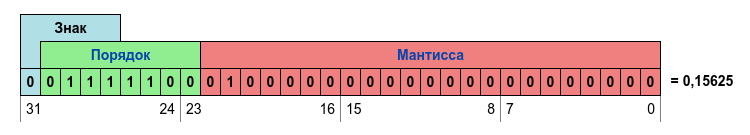
\includegraphics[width=0.9\linewidth]{\myFolder/1} \\
			Стандарт для хранения чисел с плавающей точкой. Можно почитать здесь: \href{https://ru.wikipedia.org/wiki/IEEE_754-2008}{вики}. \\
			Числа одинарной точности с плавающей запятой обеспечивают относительную точность 7-8 десятичных цифр в диапазоне от $ 10^{-38}$ до примерно $ 10^{38}$.
			Для вычисления показателя степени из восьмиразрядного поля порядка вычитается смещение порядка равное $127_{10} = 7F_{16} = 01111111_2$ (то есть, $01111100_2 - 01111111_2 = 124_{10} - 127_{10} = -3_{10}$). Так как в нормализованной двоичной мантиссе целая часть всегда равна единице, то в поле мантиссы записывается только её дробная часть. Для вычисления мантиссы к единице добавляется дробная часть мантиссы из 23-х разрядного поля дробной части мантиссы $1,01000000000000000000000_2$. Число равно произведению мантиссы со знаком на двойку в степени порядка = $1,01_2*2_{10}^{-3_{10}} = 101_2*2_{10}^{-5_{10}} = 5_{10}*2_{10}-5_{10} = 0,15625_{10}$. \\
			(Взято из \href{https://ru.wikipedia.org/wiki/%D0%A7%D0%B8%D1%81%D0%BB%D0%BE_%D0%BE%D0%B4%D0%B8%D0%BD%D0%B0%D1%80%D0%BD%D0%BE%D0%B9_%D1%82%D0%BE%D1%87%D0%BD%D0%BE%D1%81%D1%82%D0%B8}
				{другой статьи})
		\end{lecSubsection}
	\end{lecSection}
	\begin{lecSection}[Явное и неявное преобразование типов]
		\cppfile{\myFolder/2}{Неявное преобразование}{implicit_cast}
		В коде выше используется неявное преобразование: дает возможность писать код гибче, однако требует осторожнее (так, в строке 3 используется \textit{целочисленное} деление).
		\cppfile{\myFolder/3}{Не всегда удается преобразовать типы}{no_cast1}
	\end{lecSection}
	\begin{lecSection}[Типы целых чисел]
		В C++ есть несколько типов целых чисел:
		\begin{enumerate}
			\item \textbf{char} - код символа (по умолчанию 1 байт)
			\item \textbf{int} - целое число (сколько байт - не известно).
		\end{enumerate}
		Не стоит быть уверенным, что \textbf{char} - 1 байт, на разных процессорах по-разному. В C++ так устроено: язык заточен под процессор, на котором он будет выполняться. Для обоих типов можно указать \textbf{signed} и \textbf{unsigned} - знаковый тип или нет.
		\cppfile{\myFolder/sign_no_dec}{Пример доп. указателей к типам}{sign_no}. Стоит быть внимательным: сравнение для знаковых и беззнаковых может пойти не так, как хотелось бы. Пример:
		$-1 > 50$ - верное равенство, если -1 имеет тип \textbf{signed}, а 50 - \textbf{unsigned}. Проблема заключается в том, что $-1$ соответствует максимальному числу из \textbf{unsigned}.
	\end{lecSection}
	\begin{lecSection}[Логические операции]
		Работают над переменными типа \textbf{bool}.\\
		\begin{tabular}{cc}
			\multicolumn{1}{c|}{не} & $!A$ \\
			\multicolumn{1}{c|}{и} & $A\&\&B$ \\
			\multicolumn{1}{c|}{или} & $A || B$ \\
		\end{tabular}\\
		\vspace*{5pt}
		Здесь почти то же самое, что в Python, лишь синтаксис другой.
	\end{lecSection}
	\begin{lecSection}[Битовые операции C++]
		Как можно поменять две переменные без третьей? Для этого могут помочь логические операции. В C++ их несколько:
		\begin{enumerate}
			\item Инверсия -- $~x$ -- работает над \textit{любым} числом, не обязательно \textbf{bool}. Заменяет все ноли и единички в представлении числа на противоположные.
			\item Битовое \textbf{"и"} -- $x\& y$ -- умножает биты в двоичном представлении двух чисел. Иногда битовое "и" называют \textit{наложением маски}.
			\item Битовое \textbf{"или"} -- $x | y$ -- складывает биты в двоичном представлении двух чисел.
			% TODO: экранирование
			\item xor - x$\wedge$y. С его помощью можно как раз осуществить обмен переменных: \\
			x = x $\wedge$ y \\
			y = x $\wedge$ y \\
			x = x $\wedge$ y \\
		\end{enumerate}
	\end{lecSection}
	\begin{lecSection}[Автоматические типы переменных]
		\cppfile{\myFolder/auto}{Автоматический тип переменной}{auto}
		Код будет присваивать переменной х различные типы, однако этот трюк будет работать, только если компилятору сказать использовать современный стандарт (например, C++11)!
	\end{lecSection}
	
	\begin{lecSection}[Простейшие массивы]
		В C++, как и во многих языках, существуют массивы.
		\cppfile{\myFolder/array}{Пример объявления простейшего массива}{array}
		При объявлении массива надо указать его размер. По массиву можно итерироваться через обращение к элементу (точно так же, как в Питоне): A[1] -- второй элемент и так далее; нумерация идет с \textit{нуля}.\\
		 Подробнее о массивах будет рассказано на следующей лекции.
	\end{lecSection}
	
			\begin{center}
				{Исходные коды всех программ можно найти \href{https://github.com/alekseik1/cpp\_lections\_2017/tree/master/lection\%202}{здесь}}
			\end{center}
\end{lecture}
\stepcounter{lectureNo}